\documentclass[11pt, a4paper]{article}
\usepackage[paper=a4paper, left=1.5cm, right=1.5cm, bottom=1.5cm, top=1.5cm]{geometry}
%
\usepackage[utf8]{inputenc}
\usepackage[spanish]{babel}

\usepackage{amsmath}
\usepackage{subcaption}
\usepackage{placeins}
\usepackage{float}
\usepackage{hyperref}
\usepackage{csvsimple}
\usepackage{scrextend}


\usepackage{caratula/caratula}

\begin{document}

\def\runtitulo{Reconocimiento de dígitos}

\titulo{\runtitulo}
\fecha{\today}
\materia{Métodos numéricos}

\integrante{Florencia Zanollo}{934/11}{florenciazanollo@gmail.com}
\integrante{Luis García Gómez}{675/13}{garciagomezluis.94@gmail.com}

%Carátula
\maketitle
\newpage

%Abstract
\section*{\runtitulo}

\noindent En la actualidad, debido a la importancia y magnitud de los eventos deportivos, aveces es necesario un sistema de rating que funcione a pesar de tener pocos encuentros, teniendo en cuenta dificultad del adversario, pero sin bias previo. Este trabajo trata de resolución de sistemas de ecuaciones lineales en el contexto específico del \textit{Colley Matrix Method} para ranking de equipos. 
Se busca analizar la utilidad de este método, su estabilidad respecto a los límites de la aritmética finita de las computadoras y su justicia a la hora de rankear equipos. Utilizando como punto de comparación otros métodos como \textit{porcentaje de victorias} (WP) y \textit{Elo rating}, sobre los resultados de partidos de ATP 2015 y NBA 2016.
Se muestra que las características de este método lo hacen justo bajo ciertas normas y el error aritmético generado es chico.

\bigskip

\noindent\textbf{Palabras claves:} Eliminación Gaussiana, Ranking, Colley Matrix Method, Ecuaciones Lineales.

\newpage

%Indice
\tableofcontents
\newpage

% Demás secciones
\section{Introducción}
El objeto de estudio de este trabajo es el algoritmo de clasificación \textit{k-nearest-neighbors} (kNN) en combinación con la técnica de reducción de la dimensionalidad \textit{principal component analysis} (PCA) en el contexto de un \textit{optical character recognizer} (OCR), para la clasificación de dígitos manuscritos.

Vamos a presentar las implementaciones en C++ de ambos algoritmos así como los resultados obtenidos del análisis de una variación del conocido dataset MNIST.

Desde el punto de vista técnico, detallaremos el proceso que atravesamos en la búsqueda de la construcción de un estimador que nos permita realizar la clasificación descrita con la mayor precisión posible. Tomaremos en general la métrica de performance de \textit{accuracy} para medir esto.

Desde un punto de vista más cualitativo, trataremos de entender por qué obtenemos los resultados que obtenemos, cómo podemos mejorarlos o empeorarlos. Entre otras cosas, presentaremos una herramienta que nos ayudó en este análisis.

Finalmente presentaremos algunos detalles sobre la técnica de validación que utilizamos, por qué lo hacemos y qué ventajas y desventajas tiene.

\subsection{El problema general}

\textbf{kNN} es un algoritmo de clasificación (en nuestro contexto de uso) que dada una cantidad de clases con elementos representantes en un espacio $n$ dimensional, puede determinar de forma no absoluta para nuevos elementos cuya clase es desconocida, a cual de todas las presentes pertenece. Este proceso se lleva a cabo de forma trivial determinando ``la cercanía'' entre este nuevo elemento y sus $k$ vecinos más cercanos. De forma intuitiva, podríamos decir que se apoya en que los elementos parecidos van a parar a regiones parecidas de este espacio $n$ dimensional.

Determinar $k$ representa un problema dado que al ser este muy grande, puede llegarse a tener en cuenta a elementos de clases vecinas en otra región del espacio por un lado. Por otro lado, determinar la relación de ``cercanía'' implica definir una forma de medir la ``distancia''.

La distancia euclídea es la que utilizamos en este trabajo. Su elección está fundamentada en entender las complejidades que implica tenerla. Obtener la distancia de un elemento cuya clase se quiere predecir a todos los elementos cuyas clases están determinadas por comparación puede demandarnos una considerable cantidad de tiempo, debido que este proceso depende principalmente por un lado de calcular la distancia entre dos puntos en un espacio de dimensión potencialmente grande y por otro lado la cantidad de elementos en este espacio.

Es por esta razón que son útiles las técnicas de reducción de la dimensionalidad, como \textbf{PCA}. Esta nos va a permitir la \textit{extracción} de las componentes principales de una matriz (definida por nuestro dataset), mediante la transformación de la misma a un espacio de dimensión menor en el que la varianza se vea maximizada y la covarianza se anule. Luego podremos utilizar kNN con una demanda temporal menor.

Pero definir una matriz de transformación representa también un problema, dado que requiere tiempo el pasaje de una dimensión mayor a una menor (aunque este proceso solo tenga que llevarse a cabo una vez para el entrenamiento y validación del estimador), y por otro lado la elección de cuantas componentes principales $(\alpha)$ se quiere extraer representa otro problema dado que uno desconoce cuantas son aquellas que en nuestro caso nos permiten maximizar nuestra métrica de performance.

\subsection{Nuestro problema}

El dataset que tenemos consta de 42000 imágenes de 28x28 píxeles en escala entre blanco y negro en el intervalo [0, 1] por un lado y sus correspondientes 42000 clases de pertenencia por el otro. La vectorización de esta información fue propuesta por la cátedra y consiste básicamente en cambiar el \textit{shape} de cada imagen a 1x784 en el primer caso junto con la clase correspondiente por el otro.

Durante la construcción del estimador, la validación es una etapa fundamental, por lo que una parte del dataset es separada y utilizada luego para obtener, en nuestro caso, el \textit{accuracy} total. El 80\% lo utilizamos para la construcción del estimador (entrenamiento) y el otro 20\% para su validación.

De esta forma tenemos dos matrices: una de 33600x768 y otra de 8400x768, en la que cada fila representa una imagen.

Como fue mencionado antes, \textbf{la búsqueda de $k$ para kNN} representa un problema, por eso por un lado se tratará de hallar aquel que maximice nuestra métrica de performance sin PCA.

Pero por el otro lado, la búsqueda de $k$ per se, demanda tiempo, y es un tiempo que se paga en el momento de predecir un elemento, no en la construcción del estimador dada nuestra implementación. Es por eso que por otro lado utilizaremos PCA para luego aplicar kNN. Esto demanda \textbf{la búsqueda de un $(\alpha, k)$ para PCA+kNN} óptimos.

Una vez tengamos construido un estimador que pueda predecir con alto accuracy, podemos pasar a entender cómo este varía conforme manipulamos los elementos que conforman este espacio $\alpha$ dimensional.
\newpage

\section{Desarrollo}
Existen múltiples formas en las que se puede resolver algoritmicamente un sistema de ecuaciones lineales como el nuestro, del tipo $C r = b$. Con distintas complejidades al implementar y distintas características, entre ellas se encuentran:

\begin{itemize}
    \item \textbf{Eliminación Gaussiana}: Este es uno de los métodos métodos más sencillos desde el punto de vista teórico. Consiste en derivar un sistema como el nuestro en un sistema con una matriz triangular para que sea fácil de resolver. Como ventaja: es de fácil implementación; como desventaja: no todos los sistemas pueden resolverse mediante Eliminación Gaussiana sin pivoteo y es suceptible a errores numéricos. Entre otras cosas, consta con una complejidad de $O(n^3)$.
    \item \textbf{Mediante Factorización LU}: Esencialmente se apoya en el método anterior. Consiste en obtener una factorización $C = LU$ donde $L$ es triangular inferior con unos en la diagonal y $U$ es triangular superior. Como ventaja respecto a la Eliminación Gaussiana a secas es que mediante la resolución de dos sistemas de ecuaciones simples se puede lograr una complejidad de $O(n^2)$. Como desventaja: aún no todos los sistemas pueden resolverse utilizando este método sin pivoteo.
    \item \textbf{Mediante Factorización de Choleski}: Consiste en encontrar una factorización $C = LL^t$ donde $L$ es una matríz triangular inferior. Una vez se obtiene mencionada factorización se puede resolver el sistema en cuestión utilizando, al igual que antes, dos sistemas intermedios. La diferencia con los métodos previos es que hay un algoritmo que permite hallar las matrices de estos sistemas más simple sin Eliminación Gaussiana. Como ventaja: es más eficiente para representar sistemas de ecuaciones en memoria y cuenta con una complejidad de $O(n^2)$ aunque con mejores constantes que el Método de Factorización LU. Por otra parte, tiene una mayor estabilidad numérica. Como desventaja: no todos los sistemas pueden resolverse mediante este método, solo aquellos cuya matriz principal sea simétrica definida positiva.
\end{itemize}

Todos los métodos se complementan con el algoritmo de \textit{backward substitution} ($O(n^2)$) para resolver el sistema.

\subsection{Elección del algoritmo}

Nos fue requerido resolver el sistema mediante Eliminación Gaussiana, sin pivoteos. Observemos que como la matríz $C$ de nuestro sistema es \textit{simétrica definida positiva} \cite{CMMpaper} cumple con las condiciones para resolverse con cualquiera de los métodos mencionados.

\subsection{Algunas características de nuestro sistema}

Para ello, analicemos primero cómo es la matriz $C$ de nuestro sistema y por qué cumple con las condiciones para resolverse mediante el método mencionado.

\begin{itemize}
    \item \textbf{De tener solución, es única}: dado que contamos con $n = \#\{equipo\}$ ecuaciones y $n = dim(r)$ incógnitas.
    \item \textbf{Es simétrica}: ya que la cantidad de partidos jugados entre el equipo $i$ y el equipo $j$ es la cantidad de partidos jugados por el equipo $j$ e $i$.
    \item \textbf{Es estrictamente diagonal dominante}: Por definición $n_i = \sum_{j \neq i} n_{i, j}$, por lo que es claro que $|C_{i, i}| > \sum_{j \neq i}|C_{i, j}|$ ya que $C_{i, i} = 2 + n_i$.
\end{itemize}

Al ser $C$ estrictamente diagonal dominante tiene, entre otras, las siguientes propiedades:

\begin{itemize}
    \item Es no singular
    \item Sus submatrices principales también son estrictamente diagonal dominantes
\end{itemize}

Por otro lado, sabemos que si las submatrices principales de una matriz son no singulares, entonces la misma tiene factorización LU, lo que implica la correcta aplicación de la Eliminación Gaussiana sin pivoteo.

Se implica directamente que a \textbf{$C$ se le puede aplicar la Eliminación Gaussiana sin pivoteo}.

\subsection{Sobre la estabilidad numérica de la Eliminación Gaussiana sin pivoteo}

La aritmética finita de las computadoras traen aparejados problemas para representar nuestro sistema numérico. En el caso de la Eliminación Gaussiana sin pivoteo podria presentarse al realizar una división por algún elemento de la diagonal de la matriz en cuestión que esté muy cercano a cero. En tal caso cualquier error se vería amplificado. No obstante al ser $C$ una matríz estrictamente diagonal dominante y simétrica eso nos asegura tener en la diagonal el elemento más grande en módulo tanto por fila como por columna, por lo que el pivoteo parcial en un caso como este sería redundante y se logra una cierta estabilidad numérica.

No obstante, las pruebas de control sobre la implementanción acotan el error por $10^{-4}$.

\newpage

\section{Experimentación}
\documentclass[a4paper,10pt]{article}
\usepackage[utf8]{inputenc}
\usepackage{graphicx}
\usepackage{float}
\usepackage{hyperref}
\usepackage{caption}
\usepackage{subcaption}


%opening
\title{}
\author{}

\begin{document}

\section{Búsqueda de parámetros óptimos }

El principal objetivo de esta sección es encontrar los parámetros óptimos de knn y knn+pca con respecto a la accuracy. 

\subsection{Experimentación preliminar}
Este primer segmento de la sección se enfoca en generar una intuición sobre cómo reaccionan los métodos frente a distintos valores de k, alpha para ello utilizamos una partición del dataset original para poder experimentar sobre un rango bastante extenso de parámetros sin preocuparnos demásiado por la complejidad. Este primer experimento consiste en utilizar un split simple de train y validación sobre la partición previamente elegida para cada k en el caso de kNN y para cada pareja alpha, k en caso de kNN+PCA. 

\subsubsection{kNN}

\begin{figure}[h]
\begin{subfigure}{0.5\textwidth}
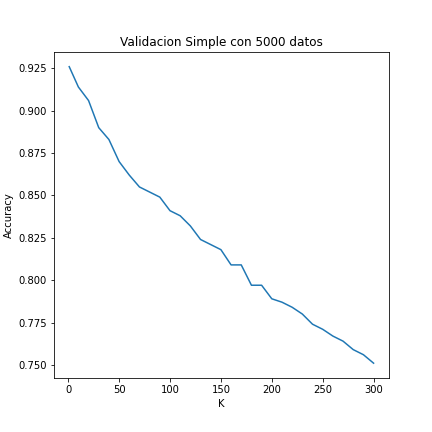
\includegraphics[width=0.9\linewidth, height=5cm]{../images/validacionSimple_knnsolo.png} 
\caption{Rango de 1-300 con granularidad 10}
\label{fig:subimbar_medio1}
\end{subfigure}
\begin{subfigure}{0.5\textwidth}
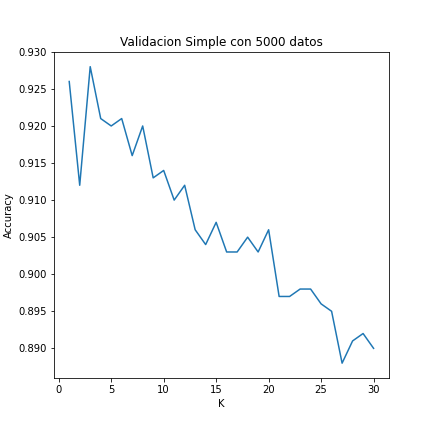
\includegraphics[width=0.9\linewidth, height=5cm]{../images/validacionSimple_knnsolo_Kchicos.png} 
\caption{Rango de 1-30 con granularidad 1}
\label{fig:subimbar_medio2}
\end{subfigure}
\caption{Validacion Simple de kNN sobre el data-set reducido.}
\label{knn_preliminar}%
\end{figure}

\par

Como podemos primer en la imagen (a) de Figura 1 muestra una presunta relación inversamente proporcional entre el k elegido y su accuracy, para vislumbrar si esto es así realizamos el mismo experimento sobre valores pequeños de k pero con más granularidad para notar cualquier variación en la accuracy, que es lo que se puede observar en la imagen (b). Ahora con más detalle se puede observar a partir de cuales magnitudes el método disminuye se eficiencia, en particular los mejores k parecen encontrarse dentro del rango 1-10.

\subsubsection{kNN+PCA}

\begin{figure}[H]
    \centering
    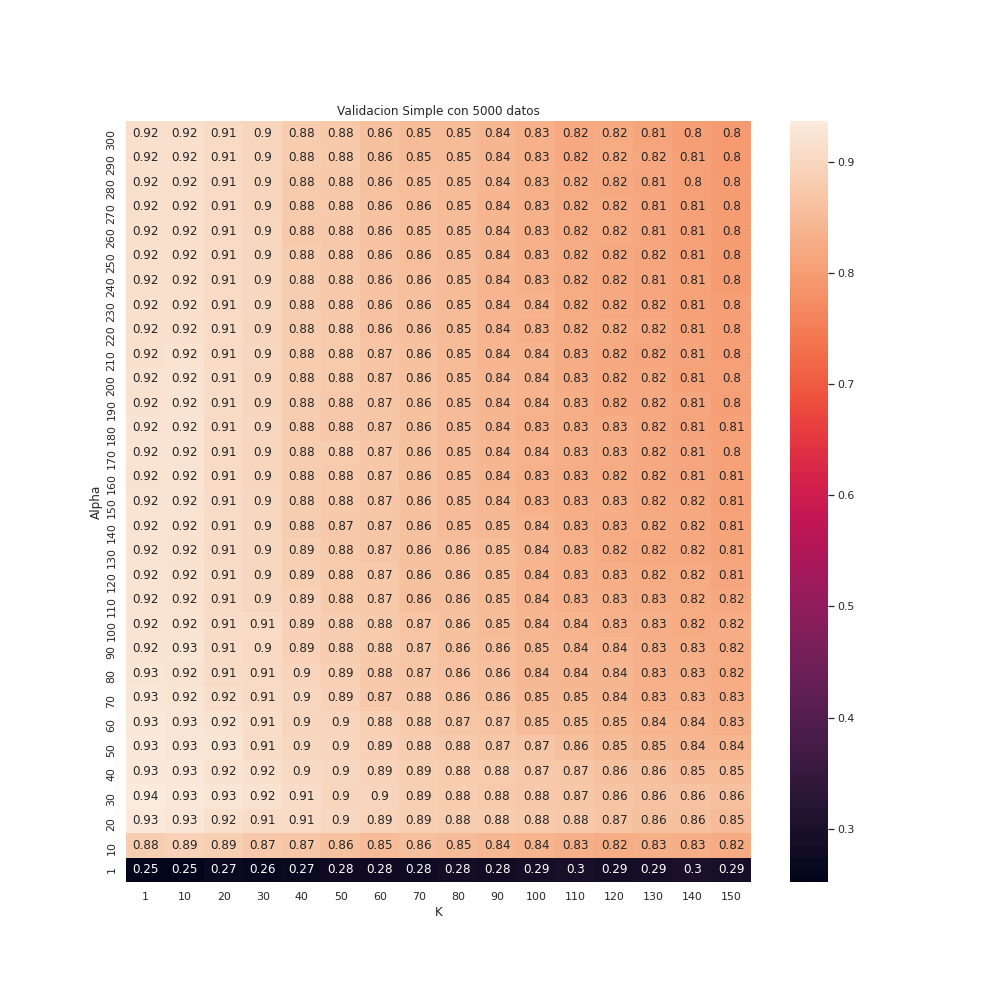
\includegraphics[width=12cm]{../images/validacionSimple_heatmap_datasetRedux}%
    \qquad
    \caption{Validacion Simple de kNN+PCA sobre el data-set reducido}
    \label{knnpca_preliminar}%
\end{figure}

Al igual que sucede en kNN podemos notar un mejor desempeño para las parejas con valores chicos de $k$, en cambio para alpha ya no estan clara la relación aunque se puede ver una leve mejora para los $alpha$ menores a 100, por esto mismo en la validacion simple que sigue sobre el dataset en su totalidad mantendremos el rango del $alpha$ y solo achicaremos el de $k$.

\subsection{Validación Simple sobre el data-set completo}

La segunda parte de esta sección realiza el mismo experimento que la primera pero ahora sobre el dataset original y eligiendo un rango condicionado por lo antes visto, con la motivación de encontrar el conjunto de los mejores diez parámetros para cada método. Notese que cuando decimos que el rango del experimento estara condicionado por una experimentacion realizada sobre un dataset reducido ,estamos asumiendo que los parámetros se ven inmutables por la cantidad de datos para entrenar y validar lo cual no es trivial por esa razon lo analizamos en la SECCION FER, donde mostramos empiricamente que esto es verdadero para nuestro caso particular.


\subsubsection{kNN}


\begin{figure}[H]
    \centering
    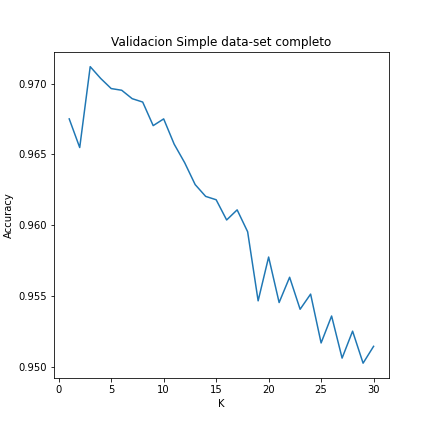
\includegraphics[width=8cm]{../images/validacionSimple_datasetCompleto.png}%
    \qquad
    \caption{Validacion Simple de kNN sobre el data-set completo}
    \label{knn_valSimple}%
\end{figure}

\begin{table}[h!]
    \begin{center}
        \begin{tabular}{|c|c|}
        \hline
        \textbf{$k$} & \textbf{accuracy} \\
        \hline
        3 &  0.9711\\
        4 & 0.9703\\
        5 & 0.9696\\
        6 & 0.9695\\
        7 &  0.9689\\
        8 & 0.9686\\
        1 & 0.9675\\
        10 & 0.9675\\
        9 & 0.9670\\
        11 & 0.9657\\
        
        \hline
        \end{tabular}
        \caption{Accuracy de las mejores 10 parejas extraido de la Validacion Simple sobre el dataset completo para kNN.}
        \label{knn_valSimple_table}
    \end{center}
\end{table}

\subsubsection{kNN+PCA}

\par

$ k \in \{1,..,80\}$ (granularidad = 2)\\$alpha \in \{  35, 160 \}$ (granularidad = 5)

\begin{figure}[H]
    \centering
    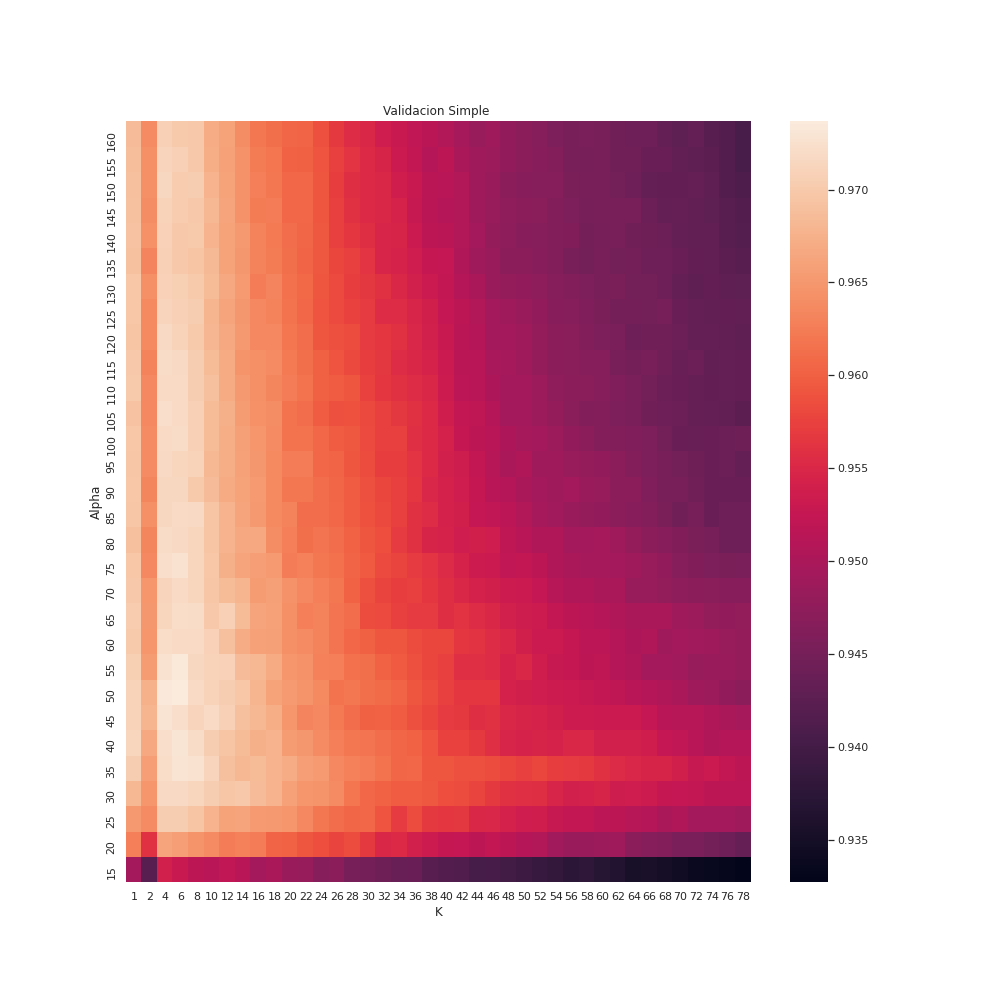
\includegraphics[width=12cm]{../images/validacionSimple_datasetCompleto_knnpca_k80}%
    \qquad
    \caption{Validacion Simple de kNN+PCA sobre el data-set completo}
    \label{knnpca_preliminar}%
\end{figure}


\begin{table}[h!]
    \begin{center}
        \begin{tabular}{|c|c|c|c|}
        \hline
        \textbf{$k$} & \textbf{$\alpha$} & \textbf{accuracy} \\
        \hline
        50 & 6 & 0.9736\\
        50 & 4 & 0.9734\\
        55 & 6 & 0.9733\\
        40 & 6 & 0.9739\\
        35 & 6 & 0.9728\\
        45 & 4 & 0.9728\\
        35 & 8 & 0.9726\\
        75 & 6 & 0.9726\\
        55 & 4 & 0.9726\\
        45 & 6 & 0.9723\\
        
        \hline
        \end{tabular}
        \caption{Accuracy de las mejores 10 parejas extraido de la Validacion Simple sobre el dataset completo para kNN+PCA.}
        \label{knnpca_valSimple_table}
    \end{center}
\end{table}

\subsection{Validación Cruzada}

Por último para conseguir el mejor parámetro o la mejor pareja en el caso de knn+pca se somete a los resultados previos a una corrida de validación cruzada ,con diez particiones, para evitar cualquier tipo de sesgo que pudiera tener nuestra anterior split de entrenamiento y validacion. 
El funcionamiento de la validación cruzada junto a la eleccion de su parámetros como diez se detalla en la seccion @LUIS.

\subsubsection{kNN}


$ k \in \{1,3,4,5,6,7,8,9,10,11\}$

\begin{table}[h!]
    \begin{center}
        \begin{tabular}{|c|c|}
        \hline
        \textbf{$k$} & \textbf{accuracy} \\
        \hline
        3 &  0.9671\\
        5 & 0.9668\\
        4 & 0.9664\\
        6 & 0.9656\\
        1 &  0.9654\\
        7 & 0.9653\\
        8 & 0.9640\\
        9 & 0.9633\\
        10 & 0.9629\\
        11 & 0.9623\\
        
        \hline
        \end{tabular}
        \caption{Accuracy promedio resultante de la Validacion Cruzada para kNN.}
        \label{knn_crossVal_table}
    \end{center}
\end{table}

\subsubsection{kNN+PCA}

En el caso de kNN+PCA  no solo tomamos las diez mejores parejas resultantes de la validación simple si no que extraemos los alpha, k de ellas y sometemos a validación cruzada a la combinacion de todos ellos parámetros.

$ k \in \{4,6,8\}$
\par
$alpha \in \{  35, 40, 45, 50, 55, 75 \}$
\begin{table}[h!]
    \begin{center}
        \begin{tabular}{|c|c|c|c|}
        \hline
        \textbf{$k$} & \textbf{$\alpha$} & \textbf{accuracy} \\
        \hline
        40 & 4 & 0.9716\\
        35 & 6 & 0.9713\\
        40 & 6 & 0.9712\\
        35 & 4 & 0.9712\\
        45 & 6 & 0.9711\\
        45 & 4 & 0.9711\\
        50 & 4 & 0.9710\\
        40 & 8 & 0.9710\\
        35 & 8 & 0.9710\\
        55 & 6 & 0.9708\\
        
        \hline
        \end{tabular}
        \caption{Accuracy de las mejores 10 parejas del total de 18 parejas extraido de la Validacion Cruzada .}
        \label{knnpca_crossVal_table}

    \end{center}
\end{table}

\subsection{ Testing sobre la mejor pareja : }


Utilizamos el 20$\%$ del data-set previamente separado para testear conseguir el $Accuracy$ de la mejor pareja.

\subsubsection{kNN}

$Accuracy_{mejor pareja} = 0.9661 $
\par
\vspace{0.5cm}
Aclaracion : la matriz de confusión se le reemplazaron los elementos de su diagonal por ceros para que sea más sencillo visualizar las demás casillas.
\begin{figure}[H]
    \centering
    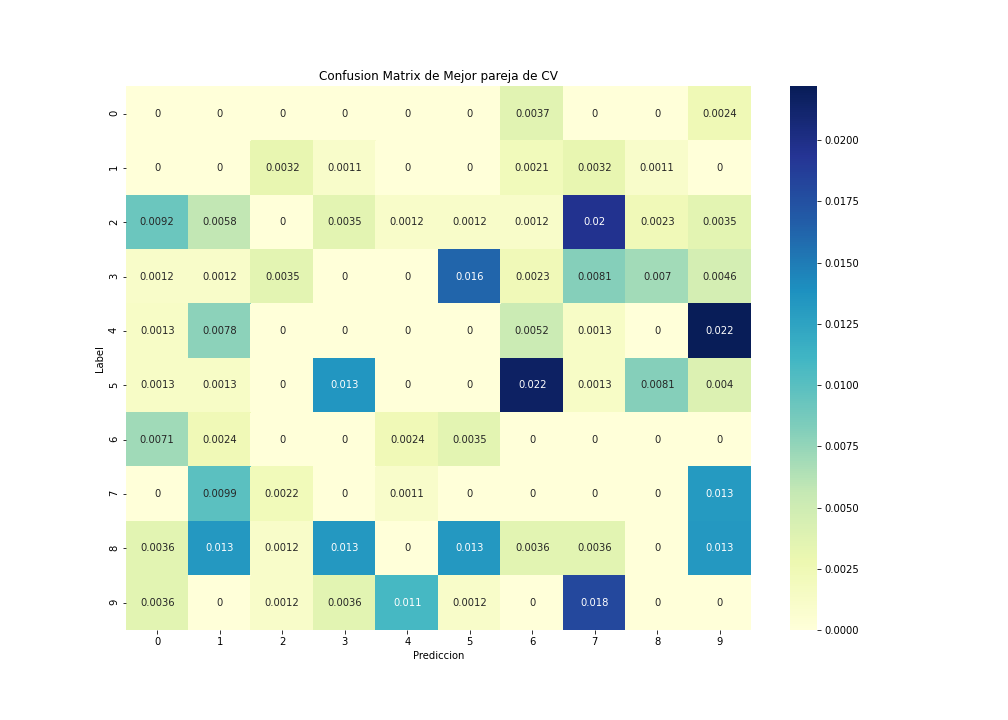
\includegraphics[width=14cm]{../images/../images/ConfMatrix_knn.png}%
    \qquad
    \caption{Matriz de Confusión para el mejor parámetro de kNN }
    \label{knn_MatrizConf}%
\end{figure}



\begin{figure}[H]
\begin{subfigure}{0.5\textwidth}
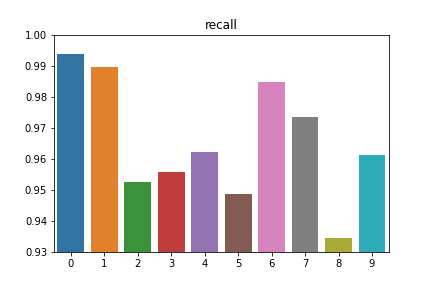
\includegraphics[width=0.9\linewidth, height=5cm]{../images/recall_knn.png} 
\caption{Recall del mejor parámetro}
\end{subfigure}
\begin{subfigure}{0.5\textwidth}
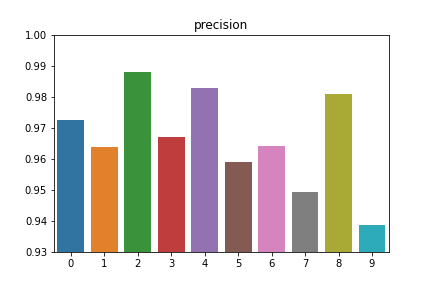
\includegraphics[width=0.9\linewidth, height=5cm]{../images/precision_knn.png} 
\caption{Precision del mejor parámetro}
\end{subfigure}
\caption{Metricas del mejor parametos para kNN.}
\label{knn_metricas}%
\end{figure}





\subsubsection{kNN+PCA}


\vspace{0.5cm}
$Accuracy_{mejor pareja} = 0.9725 $
\par
\vspace{0.5cm}
Aclaracion : la matriz de confusión se le reemplazaron los elementos de su diagonal por ceros para que sea más sencillo visualizar las demás casillas.
\begin{figure}[H]
    \centering
    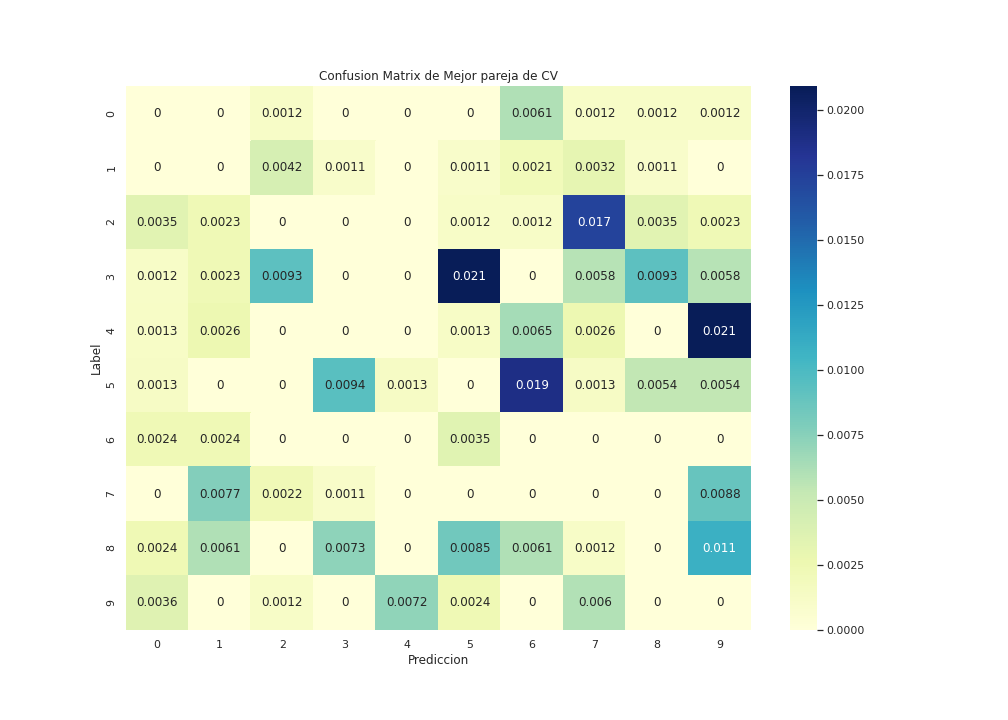
\includegraphics[width=14cm]{../images/../images/ConfMatrix_knnpca.png}%
    \qquad
    \caption{Matriz de Confusión para el mejor parámetro de kNN }
    \label{knnpca_MatrizConf}%
\end{figure}

\begin{figure}[h]
\begin{subfigure}{0.5\textwidth}
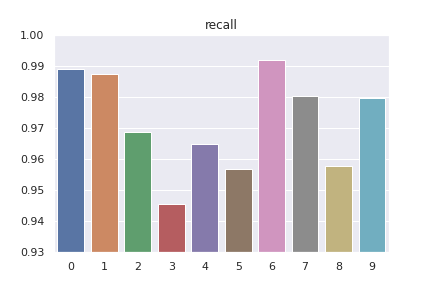
\includegraphics[width=0.9\linewidth, height=5cm]{../images/recall_knnpca.png} 
\caption{Recall de la mejor pareja}
\label{fig:metpca1}
\end{subfigure}
\begin{subfigure}{0.5\textwidth}
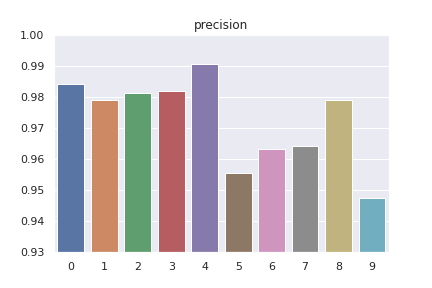
\includegraphics[width=0.9\linewidth, height=5cm]{../images/precision_knnpca.png} 
\caption{Precision de la mejor pareja}
\label{fig:metpca2}
\end{subfigure}
\caption{Metricas de la mejor pareja para kNN+PCA.}
\label{knnpca_metricas}%
\end{figure}


\subsection{Conclusión de los parámetros óptimos}


Como se puede observar tanto en las métricas y matriz de confusión de kNN como kNN+PCA para algunos dígitos estos métodos funcionan casi perfectamente (es el caso del uno y el cero), pero para otros como el tres por ejemplo su rendimiento decrece. Estas disparidades en la predicción hacen que nos planteamos algunas dudas , si estos datos mal clasificados pueden considerarse como outliers dado a q su morfología no se asemeja al dígito que dice su etiqueta o tal vez debemos modificar nuestro entrenamiento para llegar a mejorar la predicción de una clase complicado , si esto es asi tal vez se deba dejar de lado el accuracy general.
%al vez el 
%como por ejemplo tal vez con alguna elección de  parámetros en las que baje un poco el accuracy general podriamos lograr un desempeño mejor en algunos de estos dígitos complicados, otra posibilidad sería que necesitamos más datos de esos dígitos para entrenar el método y asi balancear el rendimiento de todas las clases.


\subsection{Análisis de datos malclasificados por nuestro mejor predictor}

\end{document}

\FloatBarrier
\newpage
\subsection{Balanceo y morfología}
La intención de esta sección es ver tanto cómo se comporta el OCR al contar con una base de datos de entrenamiento totalmente balanceada y desbalanceada como la morfología de los dígitos y qué consecuencias pueden traer. Como tal no realizaremos iteraciones sobre el alpha o el k, asumiendo valores fijos iguales a los ``mejores'' encontrados en las secciones anteriores.

En la tabla \ref{tab:totalDigitos} se puede ver la cantidad por digitos del dataset completo. Como el 5 (del que menos hay) tiene 3795 instancias, no podemos elegir más de esa cantidad. En todos los experimentos que siguen vamos a utilizar 3795 instancias, 2277 de entrenamiento y 1518 de validación.

\begin{table}[h]
\centering
\begin{tabular}{|c|c|}
\hline
0 & 4132 \\ \hline
1 & 4684 \\ \hline
2 & 4177 \\ \hline
3 & 4351 \\ \hline
4 & 4072 \\ \hline
5 & 3795 \\ \hline
6 & 4137 \\ \hline
7 & 4401 \\ \hline
8 & 4063 \\ \hline
9 & 4188 \\ \hline
\end{tabular}
\caption{Cantidad de instancias por dígito}
\label{tab:totalDigitos}
\end{table}

Primero vimos qué pasaba al tener un conjunto de entrenamiento totalmente balanceado. Como podemos ver en la fig.\ref{fig:bal_recall_prec} el sistema tiene bastante buena precisión y recall para cada una de las clases, con un accuracy de 0.925.
\begin{figure}[h]
    \centering
    \begin{subfigure}{.5\textwidth}
        \centering
        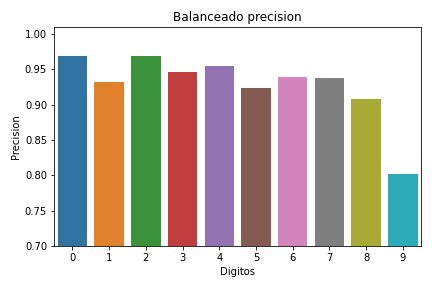
\includegraphics[width=.8\linewidth]{images/balanceo/Balanceado precision_3795.png}
    \end{subfigure}%
    \begin{subfigure}{.5\textwidth}
        \centering
        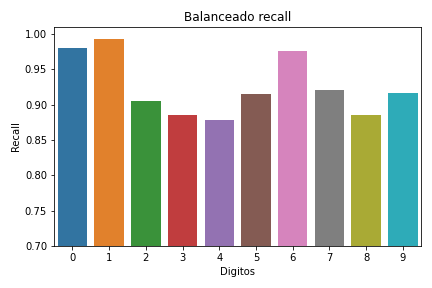
\includegraphics[width=.8\linewidth]{images/balanceo/Balanceado recall_3795.png}
    \end{subfigure}%
    \caption{Recall y precision de balanceado}
    \label{fig:bal_recall_prec}
\end{figure}

Como la precisión del 9 es la más baja intentamos mejorar esto agregando más instancias del mismo, cabe aclarar que cuando decimos agregar es en realidad un desbalance pero tenemos la misma cantidad de instancias de entrenamiento. La proporción normalizada de 9s es 0.16 y 0.093 para el resto. En la figura \ref{fig:9s_recall_prec} se ve que, contrario a lo que suponíamos, la precisión baja aún más y además empeora el recall de los 4s.
\begin{figure}[h]
    \centering
    \begin{subfigure}{.5\textwidth}
        \centering
        \includegraphics[width=.8\linewidth]{images/balanceo/Con más 9s precision_3795.png}
    \end{subfigure}%
    \begin{subfigure}{.5\textwidth}
        \centering
        \includegraphics[width=.8\linewidth]{images/balanceo/Con más 9s recall_3795.png}
    \end{subfigure}%
    \caption{Recall y precision de desbalance con más 9s}
    \label{fig:9s_recall_prec}
\end{figure}

\FloatBarrier
Pero si esto es así entonces \textit{¿Qué pasa si agregamos más 4s en vez de 9s?}. Al hacer el intento, con proporción normalizada de 0.16 para los 4s y 0.093 para el resto, vimos que mejora el recall para el 4 sin bajar tanto el del 9 y obtiene mejor accuracy general, esto se puede ver en la figura \ref{fig:4s_recall_prec}.
\begin{figure}[h]
    \centering
    \begin{subfigure}{.5\textwidth}
        \centering
        \includegraphics[width=.8\linewidth]{images/balanceo/Con más 4s precision_3795.png}
    \end{subfigure}%
    \begin{subfigure}{.5\textwidth}
        \centering
        \includegraphics[width=.8\linewidth]{images/balanceo/Con más 4s recall_3795.png}
    \end{subfigure}%
    \caption{Recall y precision de desbalance con más 9s}
    \label{fig:4s_recall_prec}
\end{figure}

\FloatBarrier
Esto tiene sentido, ya que el mayor error está cuando los valores son 4s pero clasifica erroneamente como 9, como se puede ver en \ref{fig:bal_conf}. Por ende al tener más instancias de 4s le estamos dando al sistema más vecinos para comparar del valor con el que más flaquea, esto aumenta el recall del 4 al dar menos falsos negativos, luego como el valor predecido era 9 la precisión de este último aumenta ya que hay menos falsos positivos.
\begin{figure}[h]
 \centering
 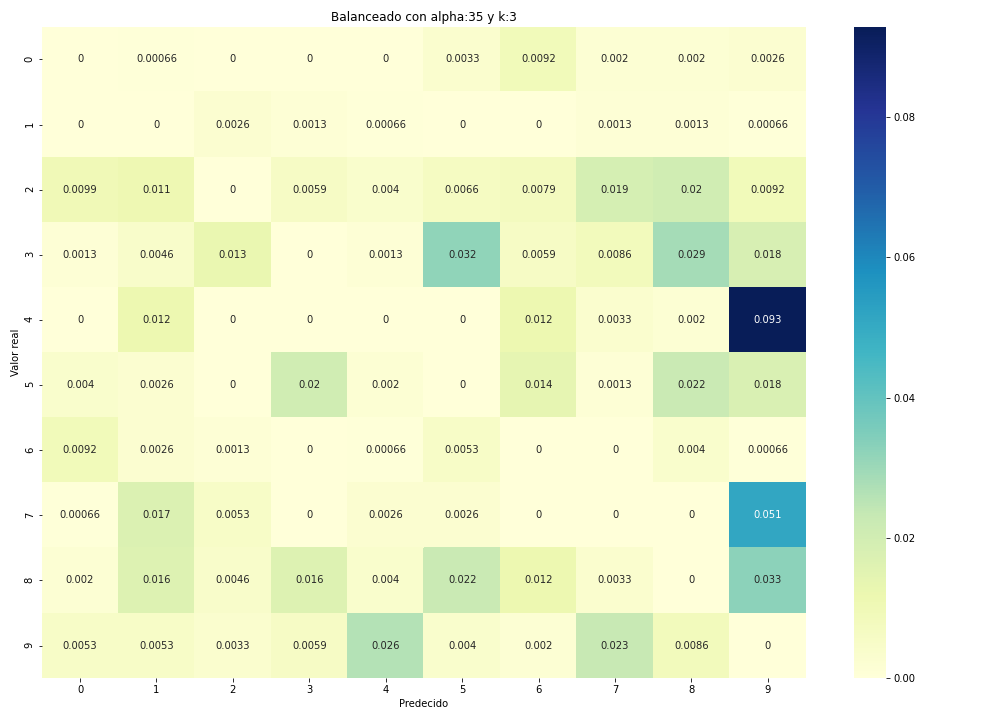
\includegraphics[width=0.8\linewidth]{images/balanceo/Balanceado con alpha:35 y k:3_3795.png}
 \caption{Matriz de confusión para dataset balanceado (diagonal anulada)}
 \label{fig:bal_conf}
\end{figure}

A modo de resúmen y para facilitar su comparación, en la figura \ref{fig:comparaciones} se puede ver la precisión, recall y f1 para cada una de las clases y cada uno de los desbalances propuestos hasta ahora.
\begin{figure}
    \centering
    \subfloat{{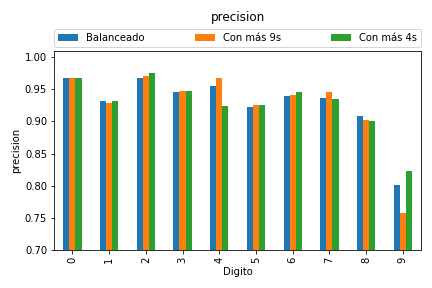
\includegraphics[width=.5\linewidth]{images/balanceo/primeros3exp_precision_3795.png} }}%
    
    \subfloat{{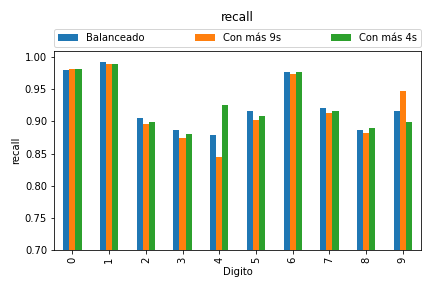
\includegraphics[width=.5\linewidth]{images/balanceo/primeros3exp_recall_3795.png} }}%
    \subfloat{{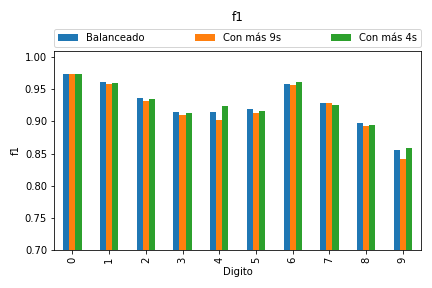
\includegraphics[width=.5\linewidth]{images/balanceo/primeros3exp_f1_3795.png} }}%
    
    \caption{Precisión, recall y f1 por clase para los primeros tres desbalances}
    \label{fig:comparaciones}
\end{figure}

\FloatBarrier

Creemos que los errores se deben a la morfología de estos números, ya que basta redondear un poco la línea del cuatro para que se confundan. De hecho, mirando a mano algunas de las imágenes (fig.\ref{fig:ejemplos_feos}) con las cuáles comete errores podemos ver casos polémicos; algunos no tienen la mejor de las calidades o están girados, otros directamente fueron mal catalogados. Cabe destacar que la última fija son dígitos manuscritos ingresados por nosotros, utilizando nuestra herramienta \textit{Coso Recognizer}\footnote{El nombre fue una joda y quedó, disculpas} la cuál se puede usar corriendo el script de mismo nombre\footnote{Está en la carpeta notebooks, requiere tkinter (apt-get install python3-tk)}.
\begin{figure}[h]
    \centering
    \subfloat{{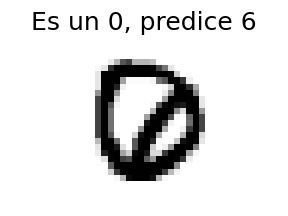
\includegraphics[width=.18\linewidth]{images/balanceo/digitosFeos/es0_pred6_4.png} }}%
    \subfloat{{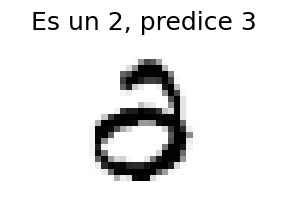
\includegraphics[width=.18\linewidth]{images/balanceo/digitosFeos/es2_pred3_1.png} }}%
    \subfloat{{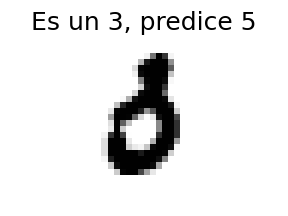
\includegraphics[width=.18\linewidth]{images/balanceo/digitosFeos/es3_pred5_9.png} }}%
    \subfloat{{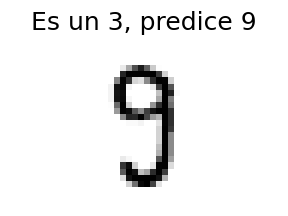
\includegraphics[width=.18\linewidth]{images/balanceo/digitosFeos/es3_pred9_3.png} }}%
    
    \subfloat{{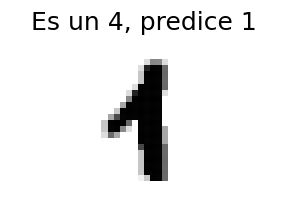
\includegraphics[width=.18\linewidth]{images/balanceo/digitosFeos/es4_pred1_1.png} }}%
    \subfloat{{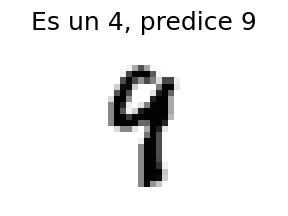
\includegraphics[width=.18\linewidth]{images/balanceo/digitosFeos/es4_pred9_9.png} }}%
    \subfloat{{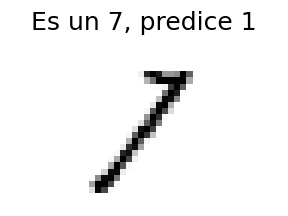
\includegraphics[width=.18\linewidth]{images/balanceo/digitosFeos/es7_pred1_0.png} }}%
    \subfloat{{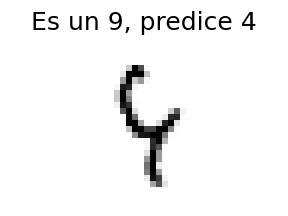
\includegraphics[width=.18\linewidth]{images/balanceo/digitosFeos/es9_pred4_0.png} }}%
    
    \subfloat{{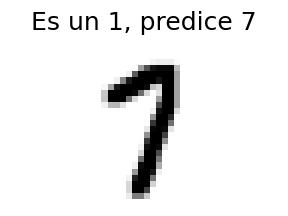
\includegraphics[width=.18\linewidth]{images/balanceo/digitosFeos/aMano_es1_pred7.png} }}%
    \subfloat{{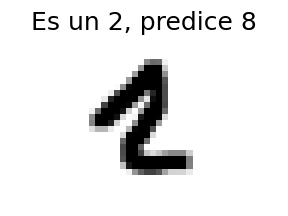
\includegraphics[width=.18\linewidth]{images/balanceo/digitosFeos/aMano_es2_pred8.png} }}%
    \subfloat{{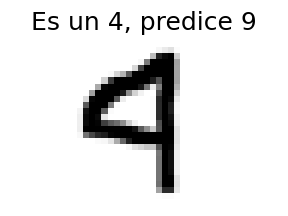
\includegraphics[width=.18\linewidth]{images/balanceo/digitosFeos/aMano_es4_pred9.png} }}%
    \subfloat{{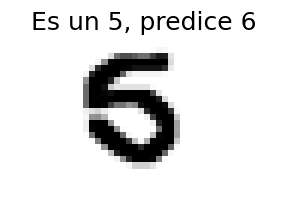
\includegraphics[width=.18\linewidth]{images/balanceo/digitosFeos/aMano_es5_pred6.png} }}%
    
    \caption{Casos horriblemente particulares}
    \label{fig:ejemplos_feos}
\end{figure}

\FloatBarrier
Hasta ahora sabemos que el desbalance no es inherentemente malo sino que podría beneficiarnos, entonces surge la pregunta \textit{¿Cuál es la configuración (proporciones de dígitos) que más accuracy genera?}

Para empeza desbalanceamos a mano utilizando como guía el recall de cada clase, en favor de los que menos poseen. Probamos con las proporciones: 

\begin{description}
 \item [Muchos 4s, más 3s] proporción de 0.11, 0.18 para el 3 y 4 (resp.) y 0.093 para el resto. 
 \item [Muchos 4s, más 3s, 7s y 8s] proporción de 0.18 para el 4, 0.11 para el 3,7 y 8 y 0.087 para el resto. 
\end{description}

En la figura \ref{fig:acc} se ve que con más 4s y 3s se obtiene aún más accuracy pero ya al desbalancear 7s y 8s volvemos a perder exactitud, aunque aún es mejor que el set balanceado.
\begin{figure}[h]
 \centering
 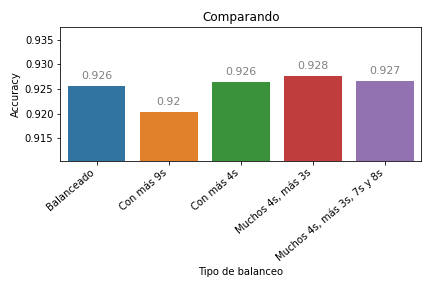
\includegraphics[width=0.65\linewidth]{images/balanceo/acc.png}
 \caption{Accuracy para cada uno de los casos.}
 \label{fig:acc}
\end{figure}
 
\FloatBarrier
Luego generamos automáticamente algunas variaciones de proporciones en función de encontrar alguno con mayor accuracy. Dividimos los dígitos en dos grupos, los del primero tienen una proporción fija y los restantes se dividen lo que queda equitativamente. Variamos la proporción fija en [0.11, 0.18, 0.19] y como grupos se tomaron todas las combinaciones de 1 y 2 elementos. Estos casos no llegaron a ser tan buenos como \textit{Muchos 4s, más 3s}, en la figura \ref{fig:accAutom} se puede ver la variación de los accuracy conseguidos.

\begin{figure}[h]
 \centering
 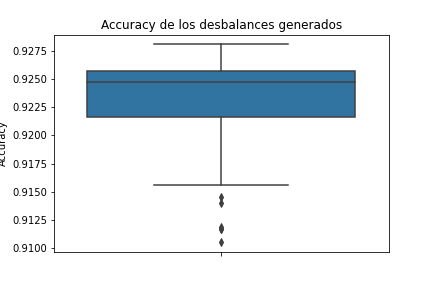
\includegraphics[width=0.65\linewidth]{images/balanceo/acc_generados.png}
 \caption{Accuracy casos generados}
 \label{fig:accAutom}
\end{figure}

\FloatBarrier


\FloatBarrier
\newpage
\subsection{Sobre Cross Validation con K-Fold}

Como fue propuesto por la cátedra, para validar que la elección de nuestros parámetros para el sistema lleven luego a una buena generalización al momento de clasificar dígitos, utilizamos la técnica de cross validation con K-Fold.

Brevemente, para el caso de KNN+PCA, por ejemplo, tenemos que elegir entre $(k_i, \alpha_i)$ óptimos, por lo que para cada par se partirá el trainset disponible en $K$ conjuntos para luego hacer $K$ pruebas, donde en cada una de ellas la unión de $K-1$ conjuntos pasan a ser un nuevo trainset y el restante pasa a ser un nuevo testset. Al menos cada conjunto fue un testset después de haber aplicado K-Fold. Luego, promediando algúna métrica de performance entre las $K$ disponibles se puede obtener el valor final para la misma, la cual puede ser comparada después con las generadas por otros pares de parámetros. Los elegidos van a poder ser validados con el testset original.

Las preguntas que se listan a continuación surgieron de pensar las cosas mencionadas en el párrafo anterior y se realizaron pruebas teniendo en cuenta los siguientes atributos:

\begin{itemize}
    \item \textbf{Métrica de performance}: Accuracy, tomando la media.
    \item \textbf{Algoritmo}: KNN+PCA
    \item \textbf{Rango de $K$}: $\{5, 10, 15, 20\}$
    \item \textbf{Rango de $k$}: $\{1\dots53, 2\}$
    \item \textbf{Rango de $\alpha$}: $\{10\dots120, 10\}$
    \item \textbf{Dataset}: Primeros 10000 elementos del dataset original, tomando el $80\%$ como trainset y el restante como testset.
\end{itemize}

\subsubsection{¿Qué valor debería tener K?}\label{KFoldValueK}

Elegir los parámetros con validación simple consiste en hacer $n$ corridas de nuestro sistema, donde $n$ es el número de parámetros candidatos que tenemos. Hacerlo con cross validation utilizando K-Fold nos lleva a realizar $n * K$ corridas del sistema, por lo que el tiempo de duración del experimento puede llegar a ser grande. Dependiendo de, entre otras cosas, el tamaño del dataset y la eficiencia general de los algoritmos.

Esto nos llevó a probar inicialmente con una serie de valores fijos para $K$ y una parte del dataset original para ver si, la métrica de performance variaba mucho, e inferir en ese caso si vale el costo temporal o no hacer la validación con valores de $K$ cada vez más altos.

\begin{itemize}
    \item \textbf{Pregunta}: ¿Será apreciable la variación de nuestra métrica de performance si K crece?
    \item \textbf{Hipótesis}: Si: incrementar $K$ permitiría ver como se comporta el sistema con $K$ trainsets distintos, por lo que es factible que mientras más trainsets existan, se van a poder elegir parámetros que generalicen mejor y maximicen la métrica de performance.
\end{itemize}

\subsubsection*{Análisis y resultado}

Para uno de los pares estudiados $(k = 3, \alpha = 40)$

\begin{figure}[H]
    \centering
    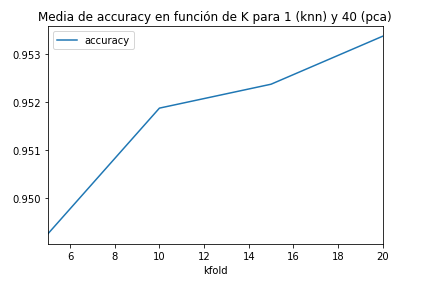
\includegraphics[scale=0.7]{images/KFoldIncreasingK.png}
    \caption{Variación del accuracy en función de $K$ para uno de los pares estudiados.}
    \label{fig:KFoldIncreasingK}
\end{figure}

Como se puede apreciar en la figura \ref{fig:KFoldIncreasingK}, efectivamente, hubo un incremento en el accuracy.

A juzgar por esta prueba, mientras mayor sea $K$, mayor es el accuracy por lo que parece conveniente, al menos tomar $K = 20$.

¿Pero que sucede si tomamos $K$ arbitrariamente grande? Podríamos decir con cierta seguridad que el sistema se encontraría overfitteado, lo que nos llevaría a tener predicciones pobres al validar.

Elegir $K$ arbitraríamente alto tampoco seria productivo.

\subsubsection{¿Qué relación hay entre K y el tamaño del trainset?}\label{KFoldTrainSizeAcc}

Para la siguiente prueba, el trainset definido de 8000 elementos, lo particionamos en cuatro trainsets: el primero de 2000, el segundo de 4000, el tercero de 6000 y el último (el completo) de 8000 elementos.

\begin{itemize}
    \item \textbf{Pregunta}: A mayor tamaño del trainset y de $K$, ¿el accuracy también será mayor?
    \item \textbf{Hipótesis}: Si: de alguna forma será mayor en proporción a la cantidad de elementos que haya en el conjunto de entrenamiento. De esta forma, la mejor elección de nuestros parámetros la vamos a poder realizar con el dataset completo (42000 elementos, 33600 para el trainset) propuesto por la cátedra.
\end{itemize}

\subsubsection*{Análisis y resultado}

La evaluación fue consistente con la hipótesis planteada, observando el par mencionado con anterioridad.

\begin{figure}[H]
    \centering
    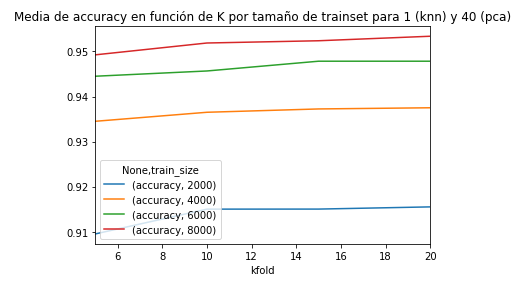
\includegraphics[scale=0.7]{images/KFoldAccTrainSize.png}
    \caption{Accuracy vs K: La mayor diferencia parece lograrse no variando K, si no variando el tamaño del trainset.}
    \label{fig:KFoldAccTrainSize}
\end{figure}

En la figura \ref{fig:KFoldAccTrainSize} se puede observar, análogamente al caso anterior que para diferentes tamaños de trainset se ven pequeñas mejoras a medida que aumenta el valor de $K$, pero la diferencia notable en el accuracy está precisamente en el tamaño de mencionado conjunto. Aunque también es llamativo ver que la diferencia de la métrica entre el conjunto de 4000 y el de 2000 elementos es mayor a la que hay entre el conjunto de 6000 y 4000 elementos, y a su vez esta es mayor a la diferencia entre el conjunto de 8000 y el de 6000 elementos, lo que nos lleva a pensar que hay un límite para la mejora por el tamaño del trainset y que entrenar nuestro sistema con el dataset completo (42000 * 0.8) puede dejar esta métrica cercano a él.

\subsubsection{¿Conviene utilizar K-Fold? ¿Cuándo no?}

Utilizar K-Fold nos resulta útil para elegir los parámetros con cierta confianza de que no van a haber mayores problemas generalizando a datos desconocidos. A cambio permitimos que la información se reorganice en cada prueba de diferentes maneras. Eso mismo puede ser prohibitivo para modelos en los que haya una componente temporal presente, dado que se pierde el sentido en la información.

\subsubsection{Finalmente: ¿qué valor debería tener K?}

Vimos en la subsección \ref{KFoldValueK} que podriamos tomar $K=20$, dado que a mayor $K$, mayor accuracy. Pero también comentamos que el aumento no parecia ser significativo para el tiempo demorado.

En \ref{KFoldTrainSizeAcc} vimos que la mayor confianza se obtiene cuando el trainset tiene un tamaño grande. Esto tiene sentido dado que se entrena el sistema con más variaciones de las que se disponen con $K$ más chicos.

De los resultados obtenidos, para la configuración de la prueba mencionada previamente, las mostraron mayor accuracy fueron:

\begin{table}[h!]
    \begin{center}
        \begin{tabular}{|c|c|c|c|}
        \hline
        \textbf{$K$} & \textbf{$k$} & \textbf{$\alpha$} & \textbf{accuracy medio} \\
        \hline
        5 & 3 & 40 & 0.95\\
        10 & 3 & 40 & 0.9507\\
        15 & 3 & 40 & 0.9516\\
        20 & 5 & 50 & 0.9522\\
        \hline
        \end{tabular}
        \caption{Accuracy medio más alto para distintas configuraciones de K-Fold.}
        \label{kfold_table_1}
    \end{center}
\end{table}

Obteniendo la configuración $(3, 40)$ un accuracy mayor a la que obtuvo el par $(5, 50)$ en el testset final ($0.9645$ vs $0.9625$ respectivamente). Una elección razonable luego, sería tomar $K=15$ para hacer las pruebas. No obstante hay que tener presente que: esto es un ejemplo sobre una porción del dataset original, y el tiempo para calcular las pruebas con ese valor de $K$ puede ser significativo, por lo que finalmente $K=10$ es la elcción que tomamos para llevarlas acabo.

\newpage

\section{Conclusiones}
Hasta ahora, analizamos CMM desde varias perspectivas.

Desde la perspectiva cuantitativa, comparamos los resultados del método utilizando diferentes matrices $C$, que representan distintas configuraciones de competencias. Llegamos a que comparando los resultados contra otra implementación más estable numéricamente no obtuvimos grandes errores absolutos. Esto puede deberse principalmente a como es una matriz $C$ \textit{de Colley} y que impacto tiene en la estabilidad numérica resolver el sistema mediante Eliminación Gaussiana sin pivoteo, la cual se detalla en la sección \ref{estabilidad_numerica}.

Desde la perspectiva cualitativa, partimos desde el planteo de casos hechos a mano, descubrimos el carácter "transitivo" del método en la sección \ref{conclusion_observaciones} y planteamos una estrategia para aprovecharlo cuando la competencia se da con ciertas características en \ref{estrategia}, entre otras cosas. Comparamos a CMM con Elo y WP mediante el análisis de los resultados de ATP 2015 y llegamos a que los tres devuelven un ranking similar al real y lo utilizamos como punto de partida para estudiar la composición de Elo y WP y contrastarlos con CMM: aunque WP es similar a CMM, sin el sesgo que mencionamos, Elo no y presentamos algunas de sus características. Complementamos esta información mirando el set de datos de NBA 2016 de la cátedra.

¿En qué ámbitos más allá de los que todo el mundo tiene acceso en el día a día podemos utilizar CMM? ¿Podemos utilizarlo para definir una nueva política de reemplazo de caché? Aunque el error absoluto en general es pequeño, ¿es suficiente una implementación como la nuestra para pedir errores aún más chicos? ¿Hubieramos obtenido resultados diferentes si las comparaciones las hubiéramos hecho con otro valor de $k$ para el algoritmo de Elo? Son algunas de las preguntas que quedan abiertas en este trabajo.
\newpage
%

%%%% BIBLIOGRAFIA
\bibliographystyle{unsrt}
\bibliography{biblio}

\end{document}
